\documentclass[a4paper]{article}

\usepackage[english]{babel}
\usepackage[utf8]{inputenc}
\usepackage{amsmath}
\usepackage{graphicx}
%\usepackage[dvipdfm]{graphicx}
%\usepackage{bmpsize}
%\usepackage[colorinlistoftodos]{todonotes}
\usepackage[margin=1.15in]{geometry}

\DeclareGraphicsExtensions{.png}

\author{
  Bouffard, Daniel\\
  \texttt{bouffard.daniel@wpi.edu}
  \and
  Green, Marc\\
  \texttt{marcgreen@wpi.edu}
}

\title{An Analysis of the Feasibility and Performance of BitTorrent as a Data Transfer Protocol in Peer to Peer Backup Systems}


\date{\today}

\begin{document}
\maketitle

\section{Background Information}
\subsection{Centralized Backup Systems}
% TODO: get reliable sources for number of users of OneDrive and Google Drive
Several popular backup systems currently in use have a centralized system design. In these systems, there are many clients that all back up their data to a central location controlled by a single entity. Common elements of these systems include a fixed amount of data storage per person, with the option to obtain more for a fee. Two of the more popular systems are Dropbox, which has over 200 million users \cite{dropboxusers}, OneDrive, with over 250 million users, and Google Drive, with over 120 million users.

There are several benefits to using a centralized backup system. The first is that it is very probable that the service will always be on, as the content is being stored on servers dedicated to that purpose. Companies who offer file backup services have the hardware resources to store redundant copies of data, should a server fail. They will also have the personnel to investigate and fix any problems with the service.

However, there are also several problems with using a centralized system to backup data. One of these problems is that there is a single point of failure, should the storage site be compromised in some way (for example, natural disasters). This is less of a problem for big companies who offer the service, as they will often have the resources to handle problems, but they still need to be taken into consideration when creating the system, at a cost to the maintainers.

Another problem with centralized systems is a matter of trust: when a user stores his or her data using a third party, the third party essentially has control of that data. Even if the third party claims to offer encryption for all data that they hold, there could still be a backdoor in the service that allows them or another entity to obtain an unencrypted version of the data. One solution to help combat this is to manually encrypt the data before sending it to the third party, but this is hardly a convenient solution.

% TODO: reliable sources for data caps and monthly/yearly fees
Finally, there are often restrictions on what can be stored using the service. This includes both the size of individual files and the amount of total data. More space is gained by paying a monthly or yearly fee, and even then the amount of space is capped at a specific size. For users who need to backup a large amount of large files, these systems are not very useful.


\subsection{Peer to Peer Networks}

A peer to peer (P2P) network is a type of distributed network model in which participants form direct connections to each other. This is in contrast to the centralized client-server network model, in which all participating clients connect to a central server to carry out their task. In peer to peer networks, each participant, or "peer", functions as both a client and a server; peers initiating a request take on the role of the client, and peers answering the request take on the role of the server.

In the client-server model, servers are expected to be always available and accessible. Peer to peer networks do not have this luxury. Instead, they experience the constant fluctuation of peers joining and leaving the network. This is called \textit{churn}. Churn complicates data storage and retrieval because there is no guarantee that a peer that has some desired data will always be available. The strategies for dealing with churn, and many other P2P-specific complications, depend on the type of overlay network a P2P application uses. We discuss churn in more detail in the \textit{Peer to Peer Backup Systems} section.
% TODO link to Peer to Peer backup systems section instead of just mentioning it

\subsubsection{Overlay Networks}

% TODO: source this?
At their foundation, peer to peer networks are implemented through overlay networks on top of existing infrastructure, such as the Internet. The responsibilities of a P2P overlay network includes providing peers the ability to join and leave the network and find other peers. 

There are three categories of overlay networks that can be used as the network abstraction on which a P2P network is built. \textit{Structured} overlay networks organize peers according to some geometry, e.g., a ring. This structure is strictly maintained as nodes join and leave the network. \textit{Unstructured} overlay networks, on the other hand, do not organize peers, but instead allow the network to grow into any shape, determined only by the routing table of each peer. \textit{Hierarchical} overlay networks are composed of multiple groups of peers each forming their own overlay network. A representative peer from each group joins a top-level overlay network, connecting the distinct groups \cite{p2pSurvey}. 

These overlay networks, and how they implement their responsibilities, are discussed below.

% For each overlay, discuss:
% - Joining
% - Finding Peers
% - Situations where each are appropriate
\hfill \\
\textit{Structured Overlay Networks}
\hfill \\

Structured overlay networks are defined by a virtual address space and a topology. For example, peers could be organized in a ring and addressed by consecutive numbers, incrementing counter-clockwise. Or, peers could be organized in a 3D cube and addressed by their (x,y,z) coordinates.
% TODO maybe insert figure of chord ring topology

The purpose of peer to peer networks (more broadly, networks in general) is to share data. The data that is present in a structured overlay network shares the same aforementioned virtual keyspace. That is, structured overlay networks map the data into a valid address through some function. For example, if peers were addressed by a hash of their IP address (which could be organized into a ring), the data could also be hashed to find its "address". This is done to determine which peer is responsible for a given piece of data. Specifically, a peer is responsible for all data in the keyspace that the peer is closest to. Thus, the size of the keyspace for which a peer is responsible decreases as more peers join the network.

% TODO cite router.bittorrent.com as well known bootstrap node?
To join a structured overlay network, a peer must know at least one other peer in the network. This peer is often called the \textit{bootstrap peer}. The joining peer will contact the bootstrap peer to find its proper place in the topology. More details are given below, in the explanation of how to \textit{find other peers}. In BitTorrent's structured overlay network \footnote{To clarify, we are referring to BitTorrent's distributed hash table, not its unstructured network. The latter involves using cenralized trackers, the former removes such dependency. We do not yet use the term \textit{distributed hash table} to keep the explanation simple without loss of generality. We discuss distributed hash tables elsewhere in the paper.}, a well known bootstrap node \footnote{The BitTorrent specification uses \textit{node} to refer to participants of its structured overlay network and \textit{peer} as a more general term \cite{bittorrentDHT}. We will adopt this convention when speaking about BitTorrent, and use them interchangably otherwise.} is router.bittorrent.com. A BitTorrent node randomly chooses a 160 bit \textit{nodeID} to use as an address. It will contact a bootstrap node to find the nodes it is closest to in the topology/address space. Closeness, in this case, is determined by taking the $XOR$ of \textit{nodeID}s; smaller values are defined as closer \cite{bittorrentDHT}.

Leaving a structured overlay network can be as simple as not responding to any messages. Some specifications leave this functionality undefined, perhaps because peers may simply shutdown instead of gracefully quitting. Such overlay networks handle node departures as node failures.

To find other peers, a peer in a structured overlay network will consult its routing table. This table is initially populated upon joining the network, and is kept up to date as peers join and leave. When a joining peer first contacts a bootstrap peer, it is unlikely that the bootstrap peer has the joining peer's direct neighbors in its routing table. This is because the routing table is designed to include many peers that are close, and only a few peers that are far. A joining peer, by asking the bootstrap node, will learn of the peers in the bootstrap peer's routing table that the joining node is close to. The joining peer will then contact these peers, ask for the same information, and learn of peers it is even closer to. This process repeats (usually in $O(\log n)$ time) until the joining node learns its direct neighbors \cite{p2pSurvey}.

Structured overlay networks excel at locating specific information very quickly. This is because their virtual address space provides full accountability of any piece of data. % mention keyword searches?

\hfill \\
\textit{Unstructured Overlay Networks}
\hfill \\

Unstructured overlay networks do not enforce any particular address space or topology on peers. Instead, the networks typically resemble random graphs. There are no standardized techniques for peers in unstructured overlay networks to find other nodes or search for data. Gnutella, for example, requires a peer to contact a bootstrap peer to initially join the network. The joining peer then sends \textit{ping} messages with increasing TTL values to the bootstrap peer, which forwards the ping to its neighbors. This continues until the joining peer has received enough \textit{pong} messages from peers willing to neighbor \cite{p2pSurvey}. % [Discuss an example of searching in unstructured networks -- see survey paper, or maybe random walk paper]

The lack of standard techniques permits a large degree of freedom in these networks. % [Talk more about this]

Unstructured overlay networks excel at finding content that is popular. This is because the search techniques are more likely to find data that exist on many peers than data that exist on fewer. Contrast this to structured overlay networks, which are good for finding unpopular data because it is easy to determine which peer is responsible for it. % mention that strucutred is _bad_ for popular data? why is it?

\hfill \\
\textit{Hierarchical Overlay Networks}
\hfill \\

\subsection{Peer to Peer Backup Systems}
Peer to Peer Backup Systems are networks that allow users to backup data without the use of a central entity. Instead, each user offers some of his or her storage space in order to use the space of others as backup locations. There are several common components of existing P2P backup systems which are described in the following sections.

\subsubsection{File Chunking}
The format in which files are stored can have an effect on the efficiency of the system. pStore and PeerStore split files up into chunks, rather than distributing files to peers in their entirety. They also use special files, called File Block Lists in pStore and Descriptors in PeerStore, that list which blocks belong to the file and where to find them in the network. This has the benefit of having data units be a fixed size that will be easy to store for any node. For example, if a peer needs to store a 10GB file, it does not need to find a peer capable of storing 10GB (which might be rare); rather, it needs to find $file\_size/chunk\_size*number\_of\_replicas$ peers. Although lowering the chunk size will increase the chances of finding a peer to store on, it is imporant to choose a reasonable chunk size, as using more nodes for storage will add more overhead in finding those nodes.

File chunking also gives the benefit of easy versioning and updating of files. When a newer version of a file is backed up, the only chunks that need to be reinserted into the network are the ones that differ from the previous version. Old versions of file chunks stay in the network, so that any full version of the file can be reconstructed by requesting the appropriate file chunks. Backup systems can also reduce the amount of storage space used by sharing identical file chunks between peers.

\subsubsection{Fairness}
Another aspect of P2P backup systems is fairness between peers. Peers need to be storing an amount of data proportional to the amount that they are backing up to other peers. This can be challenging, because untrustworthy peers can attempt to game the system to obtain free backup storage. For example, consider a simple system where each peer must offer store the same amount of data that they back up on other peers. A peer could claim that all of the storage space that it should be offering is being used by other peers, while in reality the peer has not taken in any peer's data. It is clear that a mechanism needs to be built into the system that ensures that peers store the data of each other. PeerStore handles this via a combined trading and challenge system. When a peer wants to create a backup of its data, it finds a peer to trade data with. In its request to backup data, the peer will also advertise that it is willing to store a certain amount of data. The peer that receives the request will then need to accept or reject it, and if the request is accepted the receiver will also need to request a certain amount of storage. If the original requestor accepts the offer, then the two become trading partners and will send each other data \cite{PeerStore}.

\begin{figure}
  \centering
  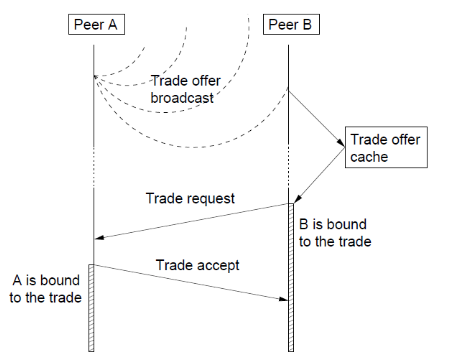
\includegraphics[scale=0.75]{PeerStoreTrading}
  \caption{Trading protocol of PeerStore}
\end{figure}

While this ensures that peers will agree to take data in proportion to the amount that they want to backup, it still does not guaratee that peers hold onto that data. For example, a peer could form a trading agreement with another peer, exchange data, and promptly discard the received data. To combat this, peers can periodically challenge peers to prove that they are actually storing data. This is the approach that PeerStore takes. A challenge in PeerStore consists of a randomly-generated number followed by a specified range of bytes in the file being backed up. The node holding the peer's data must take the bytes in the specified range, concatenate the random number with that data, take the hash of it, and return the result to the peer. If the correct answer is returned, then the node has passed the challenge. If the node does not respond or gives the wrong answer, the challenge has been failed. By choosing a random subset of bytes and creating a random number to include in the hash, the node cannot calculate the hash ahead of time and only store that; the whole file must be stored in order to be able to successfully complete all possible challenges.

\subsubsection{Churn and Data Migration}
With each storage node being regular users, it is often the case that nodes can be offline. \textit{Node churn} refers to fact that peers will continuously enter and leave the P2P network \cite{StorageSearchP2PNetworks}. The designer of a P2P backup system must take this into consideration if the system is to provide reliable access to backed up data. This has been accomplished via data migration \cite{pStore,PeerStore}, where the availability of files is periodically checked and replicas are made when the nodes being used for backup are not reliably available. Other data migration algorithms have been designed specifically to work in high churn networks \cite{StorageSearchP2PNetworks}. In this case, data replicas are periodically passed to different groups of nodes, which means that newer nodes have a chance to store data. This is beneficial because data gets evenly distributed throughout the overlay network, so any given node is not more important to the network than any others with regard to the amount of data it is storing.

The number of replicas to maintain will have an impact on the performance of the system. If the replica count is too low, the probability of recovery the entire file is lowered. If the replica count is too high, then more storage space and bandwidth will be wasted. If the system requires a peer to offer a proportional amount of storage space to the amount that it is using on other nodes, the peer will also have to offer a lot more space than what it is using locally for its own data.

\subsubsection{Cryptography}
% TODO: the figure for convergent encryption might be nice here
Since data is being stored on several untrusted peers, each user's data need to be encrypted before backup. A technique used in pStore and PeerStore is convergent encryption \cite{pStore, PeerStore}. To use this encryption mechanism, the hash of the data to encrypt is calculated, and then the hash is used as the symmetric key to encrypt the data. The main benefit of using convergent encryption is that the same data will be encrypted the same way each time, so identical blocks in the network can be shared between peers in their encrypted form.

\begin{figure}
  \centering
  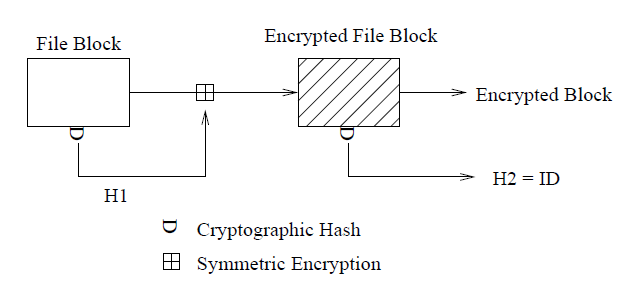
\includegraphics[scale=0.75]{ConvergentEncryption}
  \caption{Convergent Encryption from PeerStore}
\end{figure}

While this is a convenient optimization, it allows for users who have access to the unencrypted version of a file to confirm whether or not that file is being stored, since no more information is needed to encrypt or decrypt a given file.
%\subsubsection{Case Study: pStore}
%\subsubsection{Case Study: PeerStore}
\subsection{Distributed Hash Tables}

A Distributed Hash Table (DHT) is a data structure used to store (key, value) pairs in a decentralized manner \textit{DHTs share the $put$ and $get$ interface offered by hash tables, ...} DHTs are composed of multiple nodes, each responsible for a portion of the data being stored. 

% finds peers that are a part of the overlay network


\subsection{The BitTorrent Protocol}

BitTorrent is a peer to peer protocol designed for fast file sharing. A peer who wishes to share a file creates a .torrent file containing metadata about the file to be shared. This peer is known as the file's initial \textit{seeder}, and through the use of a BitTorrent client, starts \textit{seeding} the file. Peers who wish to download the file must acquire its .torrent file through an out-of-band channel, often a torrent indexer. Peers use the .torrent file to locate the initial seeder through either a centralized tracker or a DHT. These peers then connect to the initial seeder and start downloading the file. These peers are known as \textit{leechers} until they possess a full copy of the file, which is when they, themselves, become seeders.

BitTorrent can transfer files quickly due to multiple seeders each uploading different \textit{chunks} of the file to each leecher. This parallelized download is enhanced by the fact that leechers, too, upload the chunks of the file they possess to other leechers who don't have those chunks. \footnote {This is a simplified version of the BitTorrent protocol. For more information, see \cite{bittorrentProtocol}}

\subsection{BitTorrent Sync}
BitTorrent Sync is a new application developed by BitTorrent, Inc. It is a P2P synchronization tool that allows users to share files between trusted devices. This is accomplished by generating a set of 20-byte "secrets" for each folder to share and distributing the secret to each trusted device. All data is encrypted using AES-128 in counter mode \cite{btsynctech}, the key of which is derived from the secret. There are three different secrets, each of which provide different permissions for the peer that is given the secret: the read/write secret, the read only secret, and the encryption secret, which allows the node to store an encrypted version of the data, so that it cannot read the contents. A variation of the read/write and read only secrets also exists called the one-time secret, which allows a peer to send out a valid key that is only usable by one node \cite{btsyncuserguide}.

Users of BitTorrent Sync have several options for having their synced devices locate each other. The following list is taken from the BitTorrent Sync technology page \cite{btsynctech} and describes each method of peer discovery:

\begin{quote}
\begin{itemize}
\item Local peer discovery. All peers inside local network are discovered by sending broadcast packets. If there are peers with the same secret they respond to the broadcast message and connect.
\item Peer exchange (PEX). When two peers are connected, they exchange information about other peers they know.
\item Known hosts (folder settings). If you have a known host with a static ip:port, you can specify this in Sync client, so that it connects to the peer using this information.
\item DHT. Sync uses DHT to distribute information about itself and obtain the information about other peers with this secret. Sync sends SHA1(Secret):ip:port to DHT to announce itself and will get a list of peers by asking DHT for the following key SHA1(Secret)
\item BitTorrent tracker. BitTorrent Sync can use a specific tracker server to facilitate peer discovery. The tracker server sees the combination of SHA1(secret):ip:port and helps peers connect directly. The BitTorrent Sync tracker also acts like a STUN server and can help do a NAT traversal for peers so that they can establish a direct connection even behind a NAT.
\end{itemize}
\end{quote}

To allow other developers to use BitTorrent Sync as a part of their applications, the BitTorrent Sync API has been created \cite{btsyncapi}. Developers can obtain an API key by applying for one and have the application accepted by the BitTorrent Sync developers. The API key allows a developer to use all API functions, which are issued in the form of HTTP requests sent to the web interface that is started by the BitTorrent Sync executable.

BitTorrent Sync leverages the BitTorrent protocol to provide quick downloads between synced peers. We also leverage this through the use of BitTorrent Sync to provide fast recovery of backed up files. The implementation of our system is described in the next section.


\section{Implementation}
\subsection{Languages and Tools}
\subsection{System Design}
\subsubsection{Overview}
\subsubsection{}
\subsubsection{DHT}

\begin{thebibliography}{1}

\bibitem{dropboxusers} https://www.dropbox.com/news/company-info
\bibitem{pStore} pStore
\bibitem{PeerStore} PeerStore
\bibitem{StorageSearchP2PNetworks} Storage and Search in P2P Networks
\bibitem{p2pSurvey} A survey on content-centric technologies for the current Internet: CDN and P2P solutions
\bibitem{bittorrentDHT} http://www.bittorrent.org/beps/bep\_0005.html
\bibitem{btsynctech} http://www.bittorrent.com/sync/technology
\bibitem{btsyncuserguide} http://btsync.s3-website-us-east-1.amazonaws.com/BitTorrentSyncUserGuide.pdf
\bibitem{btsyncapi} http://www.bittorrent.com/sync/developers/api
\bibitem{bittorrentProtocol} http://www.bittorrent.org/beps/bep\_0003.html

\end{thebibliography}

\end{document}